\documentclass {article}
 
\usepackage{wrapfig}
\usepackage{graphicx}
\usepackage{listings}

\author{Daniel Rosso Strutz}

\title{Relatório sobre a produção do jogo BattleShips}

\begin{document}
\maketitle

\section{Introdução}
Neste documento serão discutidos os métodos e lógica utilizados para criar o jogo BattleShips.
 
\subsection{Sobre o programa}
Este programa busca emular de forma digital, o clássico jogo \textit{Batalha Naval}, que inicialmente era jogado com papel e caneta entre duas pessoas.
\subsection{Sobre este documento}
Este documento está sendo redigido em {\LaTeX} utilizando o pacote \textit{graphicx} para inserir imagens, e o pacote \textit{listings}, para citar códigos.
\section{Metódos}
O programa foi escrito em C++, porém, por falta de experiência do autor, não existem muitos pontos onde pode-se notar o uso das funções avançadas da
linguagem, invés disso, o código se assemelha muito a um código escrito em C, e pode ser transferido para essa linguagem com poucas alterações.  Faz-se uso apenas de uma biblioteca, \textit{raylib}, e de sua companheira \textit{raygui}.  Que cuida de toda a parte gráfica e de manutenção da janela, deixando para o programador apenas o trabalho de, efetivamente, implementar lógica, construindo o jogo ou utilidade desejada.
\subsection{raylib}
Conhecida por ser ``a forma mais fácil de programar um jogo de forma séria", raylib é uma biblioteca que é \emph{auto contida}, isto significa que não possui dependências extras além daquelas que já são providas por qualquer sistema relativamente moderno.

De forma resumida, o programador pode ordenar que texturas ou formatos geométricos sejam desenhados na tela sem se preocupar com qual servidor gráfico o usuário usa (\textit{wayland} ou \textit{X11}, por exemplo), assim como na famosa SDL, porém, com um formato mais simples, observe:

\begin{lstlisting}[language=c++, basicstyle=\small, caption=Rect.c]
Vector2 posicao = {
    .x = 10,
    .y = 20,
};

Rectangle exemplo = {
    .x = posicao.x,
    .y = posicao.y,
    .width = 100, 
    .height = 200, 
};

DrawRectangleRec(exemplo, BLUE); 
\end{lstlisting}

Com estes comandos, declaramos uma posição na janela (x = 10, y = 20), declaramos um retângulo com o canto superior esquerdo nesta posição, com o tamanho vertical de 200, horizontal de 100. Com a função da última linha, desenhamos esse retângulo na tela.
 
\begin{figure}[h]
\centering
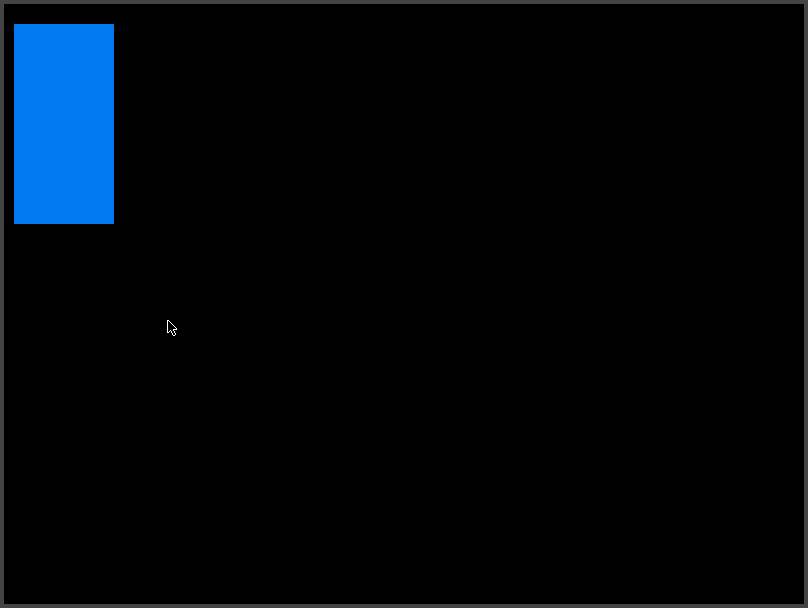
\includegraphics[width=8cm]{rectExemplo.png}
\caption{Para reproduzir o programa: \texttt{\$ make rect} no diretório do projeto.}
\end{figure}
 
Esta é apenas uma das formas de desenhar um retângulo, a biblioteca nos provê vários outros métodos, podemos checá-los analisando a header \emph{raylib.h}:

\begin{lstlisting}[language=c++, basicstyle=\small]
RLAPI void DrawRectangle
(int posX, int posY, int width, int height, Color color);
// Draw a color-filled rectangle
RLAPI void DrawRectangleV(Vector2 position, Vector2 size, Color color);
// Draw a color-filled rectangle (Vector version)
RLAPI void DrawRectangleRec(Rectangle rec, Color color);
// Draw a color-filled rectangle
RLAPI void DrawRectanglePro
(Rectangle rec, Vector2 origin, float rotation, Color color);
// Draw a color-filled rectangle with pro parameters
\end{lstlisting}

Essa citação é suficiente para referência, porém, deve ser dito que esses não são \textbf{todos} os métodos disponíveis.

\subsection{Funcionamento do código}
Perceber-se, ao examinar o programa, que há \textit{algo faltando}, isso se da ao fato de que ele foi planejado desde o começo para poder ser expandido para uma versão de dois jogadores, a implementação dessa parte está em pausa até que o projeto seja entregue. Visto que não faz parte do escopo da tarefa proposta.
 
\subsubsection{\texttt{gamePhase}s}
Após selecionar o modo de jogo no menu principal, o jogador é entra na \texttt{gamePhase==PLACE\_PHASE\_P1} e essa fase pode ser usada para explicar toda a lógica do jogo, depois disso, a fase \texttt{GAMEPLAY\_BOT} não passa de uma versão duplicada da mesma lógica, claro, aplicando regras diferentes para este modo do jogo, porém o desenho dos tabuleiros e o movimento do cursor funciona do mesmo jeito.

\subsubsection{\texttt{printBoard}}
Utilizando da lógica apresentada no programa de exemplo \texttt{rect.c}, podemos desenhar um tabuleiro, apenas multiplicando o numero de retângulos. Ao analisar o código, nota-se que não há nenhuma ligação entre o tabuleiro sendo desenhado e a matriz que efetivamente representa o tabuleiro do usuário, inclusive, \texttt{Rectangle visualBoard[BLINE][BCOL]}, é usada pra desenhar todos os tabuleiros do jogo, para isso, a função \texttt{printBoard} foi criada.
\begin{lstlisting}[language=c++, basicstyle=\small]
void printBoard
(int gamePhase, int gameBoard[BLINE][BCOL], Rectangle visualBoard[BLINE][BCOL], 
Vector2 startPos, int step, int sqSize);
//Prints the board differently depending on the state of the game;
\end{lstlisting}
Especificando qual matriz estamos desenhando, dando o valor do endereço da matriz de \texttt{Rectangle}s, a posição do primeiro quadrado, o tamanho de cada quadrado, e a distância entre a posição de um relativa ao próximo (o \textit{passo/step}), desenhamos uma matriz de quadrados na tela. Um tabuleiro.

\subsubsection{\texttt{cursor}}
Após apresentado o tabuleiro, o jogador precisa de uma forma de selecionar em que posição ele deseja colocar suas peças, ele precisa de uma representação visual de onde essas peças ficarão, e ele precisa de uma indicação da possibilidade daquela peça ser encaixada ali, para isso, é desenhado outro retângulo. Para movimentarmos ele, usamos a função \texttt{moveCursor}, que recebe todas as características visuais do tabuleiro, junto com o endereço de memória do retângulo em questão.
\begin{lstlisting}[language=c++, basicstyle=\small]
void moveCursor (Vector2 startPos, int step, int size, Rectangle *cursor);
//Moves the position of the cursor around;
\end{lstlisting}

Conforme o usuário comanda o cursor, utilizando as setas do teclado, redesenhamos ele de acordo com a ordem do jogador, implementando regras para que o cursor não saia da área de jogo. O cursor também participa ativamente do processo de colocar cada navio em seu devido lugar, pois, se sabemos em que posição o cursor está, se sabemos onde se incia o tabuleiro, podemos criar um índice que traduz diretamente para posições reais na matriz de jogo real, não apenas na visual, essa é a dinâmica que foi inventada para traduzir os movimentos do jogador.

\begin{lstlisting}[language=c++, basicstyle=\small]
Vector2 translateCursorToIndex(Rectangle *cursor, Vector2 pos, int step);
//Returns a vector with the position relative to the cursor position
\end{lstlisting}

\subsubsection{\texttt{GAMEPLAY\_BOT}}

\begin{lstlisting}[language=c++, basicstyle=\small]
step = 30; sqSize = 28;
Vector2 leftPos = {step, step * 3};
printBoard(gamePhase, p1gameBoard, visualBoard, leftPos, step, sqSize);

Vector2 rightPos = {20 + (BCOL * step) + step, leftPos.y};
printBoard(gamePhase, p2gameBoard, visualBoard, rightPos, step, sqSize);
\end{lstlisting}
 
Com a informação explicada nas últimas secções, não há qualquer dúvida sobre o que está sendo feito. É a mesma sequencia que desenha o tabuleiro, apenas duplicada e com regras aplicadas para que as duas matrizes possam caber na tela, também se incia o cursor na posição correta:
 
\begin{lstlisting}[language=c++, basicstyle=\small]
if(!cursorIsSetd){
    cursorSetUp(rightPos, step, sqSize, &cursor);
    cursorIsSetd = true;
}
moveCursor(rightPos, step, sqSize, &cursor);
DrawRectangleRec(cursor,VIOLET);
\end{lstlisting}

Todo o resto das funções são regras para que o jogo flua de forma ordenada.
Com a forma que o programa foi escrito, é possível, inclusive, demonstrar esses dois tabuleiros de forma dinâmica, e isso possibilita a futura implementação de um modo de dois jogadores.

\subsubsection{\texttt{checkWin}}
Durante a jogatina, após cada jogada, a função \texttt{checkWin} é chamada, como cada entidade no tabuleiro tem um valor específico na matriz de jogo, só precisamos checar se há algum barco ainda presente no tabuleiro.
 
\begin{lstlisting}[language=c++, basicstyle=\small]
bool checkWin(int gameBoard[BLINE][BCOL]){
for(int i = 0; i < BLINE; i++)
        for(int j = 0; j < BCOL; j++)
            if(gameBoard[i][j] == SHIP || gameBoard[i][j] == HIDDEN) return false;

return true;
}
\end{lstlisting}
 
Ao final do jogo, o jogador tem a opção de reiniciar. 
 
\section{Conclusão}
Sendo o primeiro projeto de jogo, com certeza houveram muitas oportunidades de otimização perdidas, mas o projeto serviu e ainda estás servindo como ótimo aprendizado. Uma oportunidade muito importante que foi perdida seria a implementação de uma lista encadeada para os barcos, da forma que o programa foi feito, é necessário repetir comandos para cada barco, isso poderia ter sido linearizado com uma lista, dessa forma apenas seria chamado Ship $\rightarrow$ next, até NULL.
Muitas funções foram feitas criando novas variáveis, quando podiam ser simplesmente rotinas nos endereços das variáveis antigas, isso desperdiça recursos e cria lentidão no programa, embora em momentos em que velocidade seja crucial, como no momento em que números aleatórios precisam ser \textit{forçados}, na fase \texttt{PLACE\_PHASE\_BOT}, foi tomado o cuidado para não criar e destruir variáveis a cada ciclo.

\end{document}
